\documentclass[a4paper, 12pt]{article}
\usepackage{graphicx}
\usepackage[utf8]{inputenc}
\usepackage[ukrainian]{babel}
\usepackage{amsmath}
\usepackage{fancyhdr}
\usepackage{geometry}
\geometry{top=2cm, bottom=2cm, left=3cm, right=1.5cm}
\usepackage[colorlinks=true,linkcolor=blue]{hyperref}%
\begin{document}

\begin{titlepage}
	\begin{center}
		\Large
		\textbf{Київський національний університет імені Тараса Шевченка} \\
		Факультет комп'ютерних наук та кібернетики \\

		\vspace{6cm}

		\textbf{\LARGE ЗВІТ ДО ЛАБОРАТОРНОЇ РОБОТИ №4} \\[0.5cm]
		\textbf{З дисципліни ``Чисельні методи''} \\[0.5cm]
		\textbf{Тема: Інтерполяційні методи} \\

		\vfill
		\hspace{7cm} Виконав студент 3-го курсу \\
		\hspace{7cm} групи ТТП-31 \\
		\hspace{7cm} Рісенгін Владислав \\
		\vspace{2cm}

		Київ-2024
	\end{center}
\end{titlepage}

\newpage

\hbadness=99999

\section{Постановка задачі}

Реалізувати алгоритми інтерполяції з вашого варіанту для табличної функції, отриманої з вашої аналітичної функції. Для вашої аналітичної функції на проміжку обрати не менше 15 точок, за якими побудувати табличну функцію. У звіті навести всі можливі графіки. 

Варіант 1. 
А) Метод Ньютона.
Б) Задача оберненої інтерполяції (розв’язати рівняння  для таблично заданої функції, у якості  самостійно обрати якесь число з внутрішності області значень вашої аналітичної функції на проміжку, яке при цьому не міститься в таблиці).
tg(x), x in [-0.5, 0.5]

\section{Вступ}
Інтерполяція є ключовим методом у чисельних методах для наближення значень функцій у невідомих точках на основі відомих даних.

У цій лабораторній роботі розглядаються два підходи: метод Ньютона, який використовує поліноми на основі розділених різниць, і обернена інтерполяція.

Мета роботи — реалізувати ці методи для функції $tan(x)$ та проаналізувати результати через графіки та числові значення, підтверджуючи ефективність обраних алгоритмів.

\section{Деталі реалізації}

Лабораторна робота виконана використовуючи мову програмування Python, а також бібліотеку numpy і pandas.

\clearpage
\section{Теоретичний опис методів}
\subsection{Метод Ньютона}

\begin{figure}[ht]
	\centering
	
\includegraphics[width=0.7\linewidth]{inter1.png}
\end{figure}
\begin{figure}[ht]
	\centering
	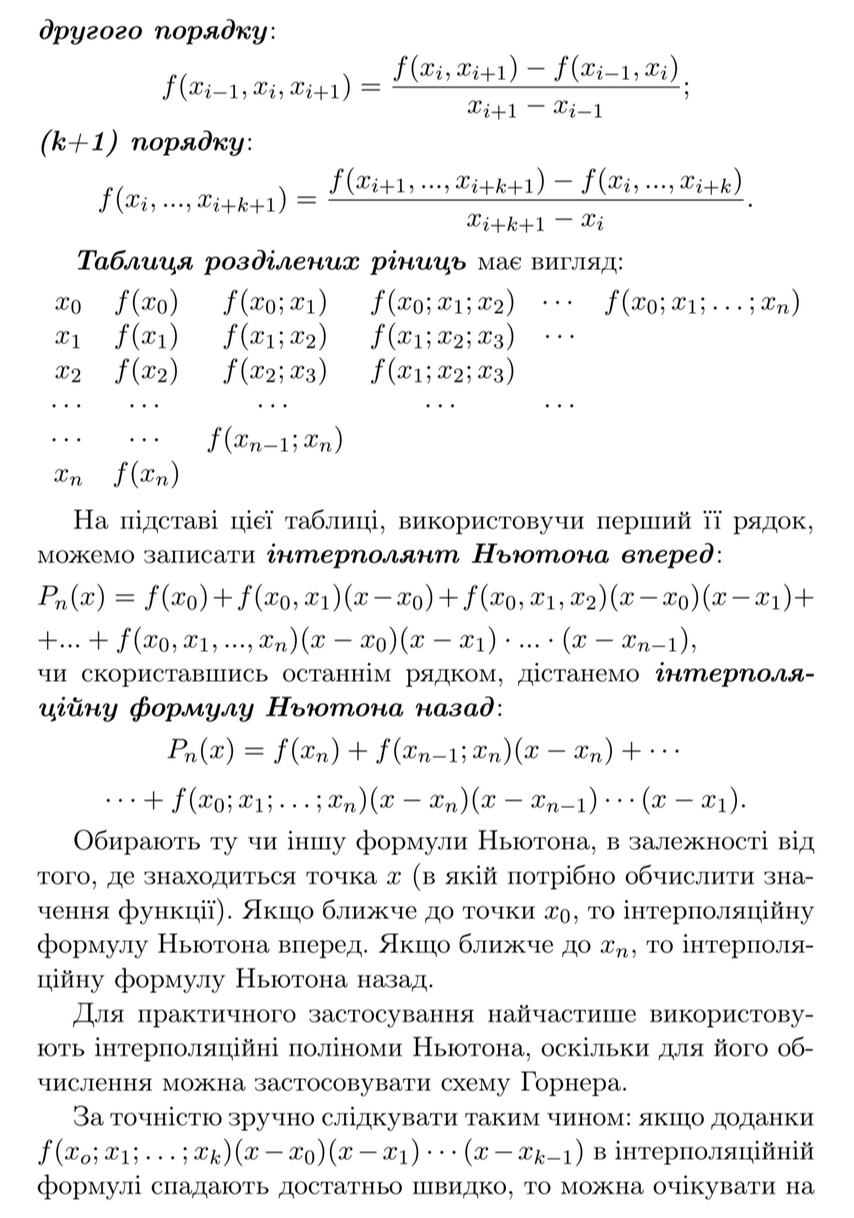
\includegraphics[width=0.7\linewidth]{inter2.png}
\end{figure}

\begin{figure}[ht]
	\centering
	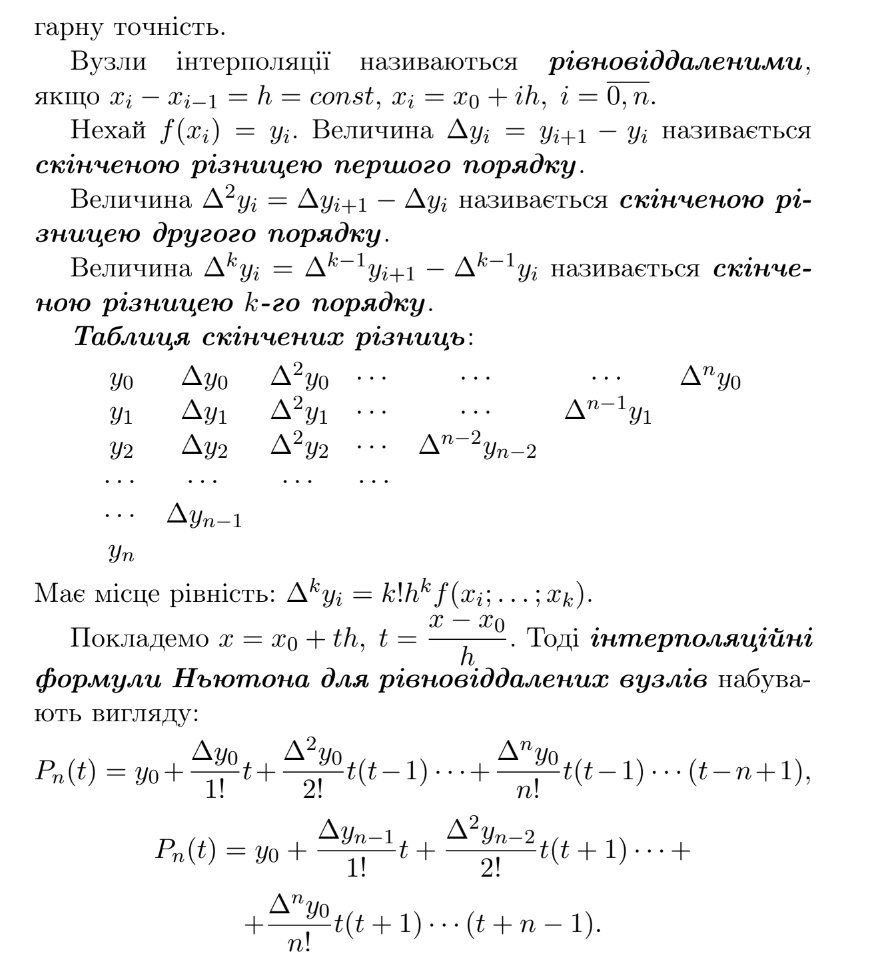
\includegraphics[width=0.8\linewidth]{inter3.png}
\end{figure}
\clearpage
\newpage

\newpage

\subsection{Обернена інтерполяція}

\begin{figure}[ht]
	\centering
	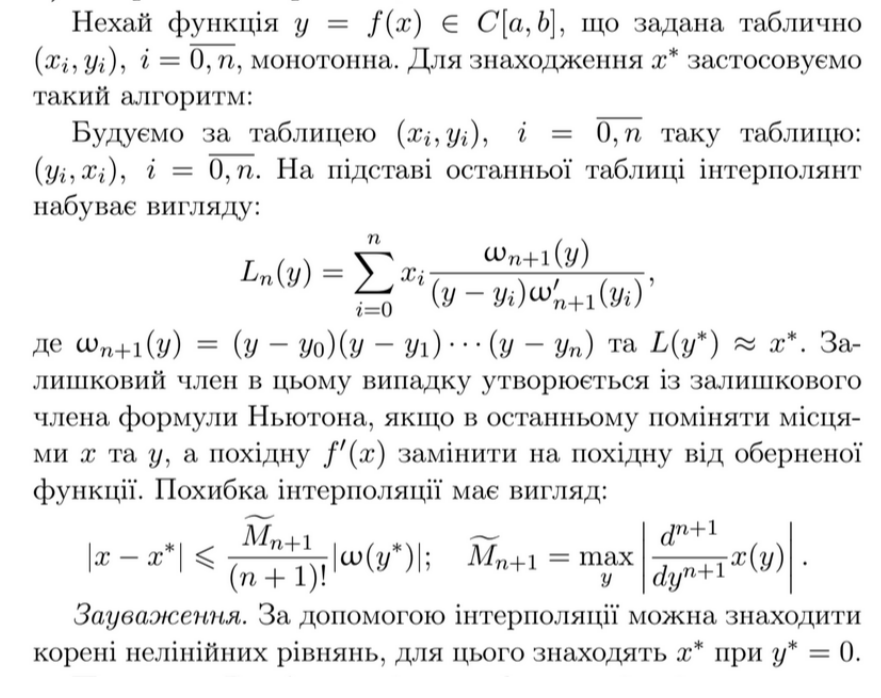
\includegraphics[width=0.8\linewidth]{rev_inter1.png}
\end{figure}

\newpage
\section{Результати роботи програми}

Лабораторна робота реалізує інтерполяційні методи для табличної функції, отриманої з аналітичної функції \( \tan(x) \) на проміжку \([-0.5, 0.5]\). Для цього було обрано 30 рівномірно розподілених точок на вказаному проміжку. 

\subsection{Таблиця розділених різниць}

Під час реалізації методу Ньютона було сформовано таблицю розділених різниць, представлена нижче:

\begin{table}[h]
    \centering
    \begin{tabular}{|c|c|c|c|c|c|c|c|c|c|c|}
        \hline
        \textbf{i} & \( x \) & \( f(x_0, \ldots, x_0) \) & \( f(x_0, \ldots, x_1) \) & \( f(x_0, \ldots, x_2) \) & \( f(x_0, \ldots, x_3) \) & \ldots & \( f(x_0, \ldots, x_{29}) \) \\
        \hline
        0 & -0.500000 & -0.546302 & 1.274935 & -0.629790 & 0.696756 & \ldots & 78.002403 \\
        1 & -0.465517 & -0.502339 & 1.231501 & -0.557712 & 0.628951 & \ldots & 0.000000 \\
        2 & -0.431034 & -0.459874 & 1.193038 & -0.492648 & 0.571533 & \ldots & 0.000000 \\
        3 & -0.396552 & -0.418734 & 1.159062 & -0.433524 & 0.522926 & \ldots & 0.000000 \\
        4 & -0.362069 & -0.378767 & 1.129164 & -0.379428 & 0.481860 & \ldots & 0.000000 \\
        \hline
		\ldots & \ldots & \ldots & \ldots & \ldots & \ldots & \ldots & \ldots \\
        \hline
        29 & 0.500000 & 0.546302 & 0.000000 & 0.000000 & 0.000000 & \ldots & 0.000000 \\
        \hline
    \end{tabular}
    \caption{Таблиця розділених різниць для функції \( \tan(x) \)}
\end{table}

\begin{quote}
\textit{Поліном :} 
\end{quote}

\begin{quote}
1.2749 * \( x^1 \) + -0.6298 * \( x^2 \) + 0.6968 * \( x^3 \) + -0.4916 * \( x^4 \) + 0.4368 * \( x^5 \) + -0.3200 * \( x^6 \) + 0.2554 * \( x^7 \) + -0.1834 * \( x^8 \) + 0.1363 * \( x^9 \) + -0.0943 * \( x^{10} \) + 0.0661 * \( x^{11} \) + -0.0439 * \( x^{12} \) + 0.0291 * \( x^{13} \) + -0.0179 * \( x^{14} \) + 0.0094 * \( x^{15} \) + 0.0007 * \( x^{16} \) + -0.0194 * \( x^{17} \) + 0.0628 * \( x^{18} \) + -0.1646 * \( x^{19} \) + 0.3880 * \( x^{20} \) + -0.8354 * \( x^{21} \) + 1.6345 * \( x^{22} \) + -2.8578 * \( x^{23} \) + 4.3016 * \( x^{24} \) + -5.0420 * \( x^{25} \) + 2.7506 * \( x^{26} \) + 7.0514 * \( x^{27} \) + -31.2570 * \( x^{28} \) + 78.0024 * \( x^{29} \)
\end{quote}

\subsection{Обернена інтерполяція}

Для оберненої інтерполяції було вибрано значення \( y = 0.18 \). Розв'язок рівняння дає:

\begin{quote}
\textit{Значення \( x \) для \( y = 0.18 \):} 0.17809283896009326
\end{quote}

Перевірка:

\begin{quote}
\( f(0.17809283896009326) = 0.17999989751251377 \)
\end{quote}


\newpage
\section{Висновок}

У результаті виконання лабораторної роботи було реалізовано інтерполяційні методи, зокрема метод Ньютона та обернена інтерполяція, \\
для функції $tan(x)$ на проміжку $[-0.5, 0.5]$. 

З отриманих результатів видно, що метод Ньютона достатньо точний.

У процесі оберненої інтерполяції вдалося знайти значення $x$ для заданого $y=0.18$.
Загалом, результати роботи свідчать про ефективність використаних алгоритмів для інтерполяції функцій.
\end{document}
